% SVN info for this file
\svnidlong
{$HeadURL$}
{$LastChangedDate$}
{$LastChangedRevision$}
{$LastChangedBy$}

\chapter{Connessione e compattezza}
\labelChapter{Connessocompatto}

\begin{introduction}
‘‘\emph{Lisa}: Allora, dov'è mio padre?\\
\emph{Professor Frink}: Beh, sarebbe ovvio anche per l'individuo più scriteriato, laureato e con specializzazione in Topologia iperbolica, che Homer Simpson è piombato... nella terza dimensione. [...] \emph{\textbf{[disegna sulla lavagna]}} Ecco un comunissimo quadrato—\\
\emph{Commissario Winchester}: Ehi ehi, rallenta, capuepopolo!\\
\emph{Professor Frink}: —ma supponiamo di estendere il quadrato oltre le due dimensioni del nostro universo, lungo l'ipotetica asse z, qui. \emph{\textbf{[tutti sussultano]}} Così si ottiene un oggetto tridimensionale noto come “cubo”, o meglio “Frinkaedro”, in onore dello scopritore!
\begin{flushright}
	\textsc{I Simpson,} La paura fa novanta VI.
\end{flushright}
\end{introduction}
\lettrine[findent=1pt, nindent=0pt]{L}{e} due proprietà che danno il nome a questo capitolo sono estremamente importanti, in quanto sono due dei principali \textit{invarianti} studiati in topologia. Entrambe rappresentano una \textit{generalizzazione} di alcuni aspetti affrontati più o meno esplicitamente durante lo studio dell'Analisi:
\begin{itemize}
	\item Ci sono sottoinsiemi del piano i cui punti possono essere \textit{connessi} da una linea arzigogolata, una spezzata o un segmento, mente
	\item Ci sono sottoinsiemi \textit{limitati} le cui successioni di punti \textit{convergono} nel sottoinsieme.
\end{itemize}
Vedremo che la \textbf{connessione} e la \textbf{compattezza} sono definite in modo abbastanza basilare, seppur non necessariamente siano intuitive a primo acchito. Tuttavia, proprio in virtù di questa semplicità, sono applicabili in tanti contesti diversi; in particolare, la compattezza come la definiremo ci permetterà di prendere informazioni note \textit{localmente} ed estenderle in modo che valgano globalmente in tutto lo spazio.
\section{Connessione}
\begin{definition}{}[Spazio connesso e spazio sconnesso]
Uno spazio topologico $X$ si dice \textbf{connesso}\index{spazio!connesso} se gli unici sottoinsiemi aperti e chiusi sono $\emptyset,\ X$. Uno spazio non connesso si dice \textbf{sconnesso}.
\end{definition}
\begin{lemma}{}[Condizioni equivalenti della sconnessione; Manetti, 4.2]\label{sconnesso}
Sono condizioni equivalenti:
\begin{enumerate}
	\item $X$ è \textit{sconnesso}.
	\item $X=A\cup B$ con $A,\ B$ aperti, non vuoti, disgiunti.
	\item $X=A\cup B$ con $A,\ B$ chiusi, non vuoti, disgiunti.
\end{enumerate}
\end{lemma}
\begin{proof}{n}~{}\\
$2\iff3)$ Se $A$ è aperto e disgiunto da $B$ tale che $X=A\cup B$ significa che $B=\mathcal{C}A=X\setminus A$ e dunque $B$ chiuso; analogamente per $B$ aperto si ha che $A$ è chiuso: allora $A,\ B$ chiusi e aperti propri.\\
$1\implies2)$ Esiste $A\neq \emptyset, X$ con $A$ aperto e chiuso. Allora basta porre $B\coloneqq\mathcal{C}A=X\setminus A$: è aperto e chiuso, è disgiunto da $A$ e tale per cui $B\neq \emptyset, X$; $A$ e $B$ soddisfano la tesi.\\
$2\implies1)$ Essendo $A, B$ aperti, si ha che $A$ è chiuso perché $A=\mathcal{C}X=X\setminus B$. Inoltre, essendo $A,B$ non vuoti, allora $A\neq X$. Dunque $A$ è aperto, chiuso e $A\neq \emptyset,\ X$ e pertanto soddisfa la tesi: esiste un sottoinsieme aperto e chiuso che non è il vuoto o l'insieme stesso.\qedhere
\end{proof}
\begin{tipsandtricks}{n}
	Il lemma \ref{sconnesso} (Manetti, 4.2) ci dice che è sufficiente trovare \textit{solo due} aperti (o chiusi) che soddisfano la condizione di cui sopra per affermare la sconnessione. Viceversa, per dimostrare la connessione, dobbiamo dimostrare che \textit{per ogni coppia} di aperti (o chiusi) non vuoti, la cui unione è $X$, essi non siano disgiunti.
\end{tipsandtricks}
\begin{example}{pn}[Spazi topologici \textit{sconnessi} in topologia Euclidea]~{}
	\begin{itemize}
		\item $X=\R\setminus\left\{0\right\}=\left(-\infty,\ 0\right)\cup \left(0,\ +\infty\right)$.
		\item $X=\unint\cup \left(2,\ 3\right)$.
	\end{itemize}
\end{example}
\begin{lemma}{}[Connesso è disgiunto o sottoinsieme di un aperto/chiuso; Manetti, 4.4]\label{connessodisgiuntoosottoinsieme}
Sia $X$ spazio topologico e $A\subseteq X$ con $A$ aperto e chiuso. Sia $Y\subseteq X,\ Y$ connesso. Allora $Y\cap A=\emptyset$,cioè $Y\subseteq Y\setminus A$, oppure $Y\subseteq A$.
\end{lemma}
\begin{proof}{n}
Consideriamo $Y\cap A$: esso è aperto e chiuso perché intersezione di due aperti e chiusi per ipotesi, in quanto $Y$ è aperto e chiuso per connessione. Essendo $Y$ connesso, un suo sottoinsieme aperto e chiuso o è l'insieme vuoto oppure è l'insieme stesso, cioè $Y\cap A=\emptyset$, cioè $Y\subseteq Y\setminus A$, oppure $Y\cap A=Y$, cioè $Y\subseteq A$.\qedhere
\end{proof}
\begin{theorem}{}[Connessione di ${\unint}$; Manetti, 4.6]
Con la topologia Euclidea, $X=\unint$ è connesso.
\end{theorem}
\begin{proof}{n}
Supponiamo che $X=\unint=C\cup D$ con $C,\ D$ entrambi chiusi. Dobbiamo dimostrare che $C,\ D$ \textit{non} sono disgiunti, ossia $C\cap D\neq 0$. Supponiamo sia $0\in C$ e poniamo $d=\inf D$. Essendo $D$ un chiuso, $d\in \overline{D}=D$.
\begin{itemize}
	\item Se $d=0$, $d\in C\cap D\neq \emptyset$.
	\item Se $d>0$ allora $\left[0,\ d\right)\subseteq C$ perché \textit{non sta} in $D$. Il passaggio alla chiusura mantiene l'inclusione, dunque $\left[0,\ d\right]\subseteq \overline{C}=C$. Segue che $d\in C$ e dunque $C\cap D\neq \emptyset$.\qedhere
\end{itemize}
\end{proof}
\begin{theorem}{}[Immagine continua di un connesso è un connesso; Manetti, 4.7]
	L'immagine continua di un connesso è un connesso, ossia
	\begin{equation*}
		\funct{}[f]{X}{Y}\text{ continua},\ X\text{ connesso}\implies f\left(X\right)\text{ connesso}
	\end{equation*}
\end{theorem}
\begin{proof}{n}
	Sia $Z\subseteq f\left(X\right)$, con $Z$ aperto e chiuso non vuoto in $f\left(X\right)$. Per dimostrare che $f\left(X\right)$ sia connesso ci è sufficiente dimostrare che $Z=f\left(X\right)$: in questo modo gli unici aperti e chiusi sono i sottoinsiemi impropri. Siccome $Z$ aperto e chiuso, esistono $A$ aperto in $Y$, $C$ chiuso in $Y$ tali che
	\begin{equation*}
		A\cap f\left(X\right)=Z=C\cap f\left(X\right).
	\end{equation*}
Allora si ha
\begin{align*}
	f^{-1}\left(Z\right)&=f^{-1}\left(A\right)\cap f^{-1}\left(f\left(X\right)\right)=f^{-1}\left(A\right)\\
	f^{-1}\left(Z\right)&=f^{-1}\left(C\right)\cap f^{-1}\left(f\left(X\right)\right)=f^{-1}\left(C\right),
\end{align*}
ossia $f^{-1}\left(Z\right)$ è contemporaneamente uguale alla controimmagine continua di un aperto e di un chiuso in $Y$, ossia è aperto e chiuso in $X$. Notiamo inoltre che, essendo $Z\neq \emptyset$, allora $f^{-1}\left(Z\right)\neq \emptyset$: essendo $X$ connesso per ipotesi, necessariamente $f^{-1}\left(Z\right)=X$.\qedhere
\end{proof}
\begin{remark}{n}
Dal teorema precedente segue che essere connesso è una proprietà topologica! Infatti, se vale per una qualunque funzione continua $\funct{}[f]{X}{Y}$, allora varrà anche per omeomorfismi tra $X$ e $Y$; in particolare, si avrà per suriettività che $f\left(X\right)=Y$ connesso.
\end{remark}
\subsection{Connessione per archi}
\begin{definition}{}[Arco]
Un \textbf{arco}\seeonlyindex{arco}{cammino} o \textbf{cammino}\index{cammino} $\alpha$ da un punto $x$ a un punto $y$ in uno spazio topologico $X$ è una funzione continua che parametrizza un \textit{percorso} finito fra gli estremi $x$ e $y$:
\begin{equation*}
\funct{}[\alpha]{\unint}{X} \text{ continua}\ \colon \alpha\left(0\right)=x,\ \alpha\left(1\right)=y
\end{equation*}
\end{definition}
\begin{definition}{}Connessione per archi]
Uno spazio topologico $X$ si dice \textbf{connesso per archi} o \textbf{c.p.a.}\index{spazio!connesso per archi}\seeonlyindex{spazio!c.p.a.}{spazio!connesso per archi} o \textbf{path-connected} se per ogni coppia di punti in $X$ esiste un arco che li collega:
\begin{equation*}
\forall x,\ y\in X\ \exists \funct{}[\alpha]{\unint}{X} \text{ continua}\ \colon \alpha\left(0\right)=x,\ \alpha\left(1\right)=y
\end{equation*}
\end{definition}
\begin{theorem}{n}[$X$ c.p.a. implica $X$ connesso; Manetti, 4.7]
\end{theorem}
\begin{proof}{n}
	Sia $X=A\cup B$, con $A,\ B$ aperti non vuoti. Vogliamo dimostrare che $A\cap B\neq \emptyset$. Essendo non vuoti, prendiamo $a\in A,\ b\in B$. In quanto $X$ è c.p.a., esiste il cammino continuo $\funct{}[\alpha]{\unint}{X}$ tale che $\alpha\left(0\right)=a,\ \alpha\left(1\right)=b$. Studiamo la controimmagine di $\alpha$:
	\begin{equation*}
		\unint=\alpha^{-1}\left(X\right)=\alpha^{-1}\left(A\cup B\right)=\alpha^{-1}\left(A\right)\cup \alpha^{-1}\left(B\right)
	\end{equation*}
Si nota che $\alpha^{-1}\left(A\right),\ \alpha^{-1}\left(B\right)$ sono entrambi aperti e non vuoti in quanto controimmagini continue di aperti non vuoti ($0\in \alpha^{-1}\left(A\right),\ 1\in \alpha^{-1}\left(B\right)$). Poiché $\unint$ è connesso, allora le controimmagini trovate \textit{non} sono disgiunte. Segue allora che $\exists t\in \alpha^{-1}\left(A\right)\cap \alpha^{-1}\left(B\right)$ e quindi:
\begin{equation*}
\alpha\left(t\right)\in\alpha\left(\alpha^{-1}\left(A\right)\cap \alpha^{-1}\left(B\right)\right)\subseteq\alpha\left(\alpha^{-1}\left(A\right)\right)\cap\alpha\left(\alpha^{-1}\left(B\right)\right)=A\cap B\qedhere
\end{equation*}
\end{proof}
\begin{theorem}{}[Immagine continua di uno spazio c.p.a. è un c.p.a.]
	L'immagine continua di uno spazio c.p.a. è c.p.a.:
	\begin{equation*}
		\funct{}[f]{X}{Y}\text{ continua},\ X\text{ c.p.a.}\implies f\left(X\right)\text{ c.p.a.}
	\end{equation*}
\end{theorem}
\begin{proof}{n}
	Considerati $y,\ z\in f\left(X\right)$, vogliamo trovare un cammino tra i due punti. Poiché $y,\ z\in f\left(X\right)$, consideriamo $a,\ b\in X$ tali che $y=f(a)$ e $z=f(b)$. Poichè $a,\ b\in X$ c.p.a., esiste un cammino $\alpha$ tale per cui $\alpha\left(0\right)=a$ e $\alpha\left(1\right)=b$. Presa ora la composizione $f\circ \alpha$ con la funzione $f$,
	\[
	\begin{tikzcd}
		{f\circ \alpha\ \colon \unint} \arrow[r, "\alpha"] & X \arrow[r, "f"] & Y,
	\end{tikzcd}
	\]
	la funzione ottenuta è continua perché composizione di funzioni continue e inoltre
	\begin{align*}
		\left(f\circ \alpha\right)\left(0\right)&=f\left(\alpha\left(0\right)\right)=f\left(a\right)=y\\
		\left(f\circ \alpha\right)\left(1\right)&=f\left(\alpha\left(1\right)\right)=f\left(b\right)=z
	\end{align*}
	Dunque $f\circ \alpha$ è un cammino fra due punti $y,\ z$ arbitrari in $f\left(X\right)$ e pertanto $f\left(X\right)$ è c.p.a.\qedhere
\end{proof}
\begin{remark}{n}
	Essere c.p.a. è invariante topologico.
\end{remark}
\begin{definition}{}[Giunzione di cammini]
	Dati due cammini in uno spazio $X$:
	\begin{gather*}
		\funct{}[\alpha]{\unint}{X}\quad \alpha\left(0\right)=x,\ \alpha\left(1\right)=y\\
		\funct{}[\beta]{\unint}{X}\quad \beta\left(0\right)=y,\ \beta\left(1\right)=z
	\end{gather*}
	Allora possiamo creare un cammino $\alpha \ast \beta$ con la \textbf{giunzione di cammini}\index{cammino!giunzione di cammini}:
	\begin{equation}
		\left(\alpha\ast\beta\right)\left(t\right)=\begin{cases}
			\alpha\left(2t\right)\quad\text{se }0\leq t\leq \frac{1}{2}\\
			\beta\left(2t-1\right)\quad\text{se }\frac{1}{2}\leq t\leq 1\\	
		\end{cases}
	\end{equation}
\end{definition}
\begin{lemma}{}[Unione di c.p.a. non disgiunta è c.p.a.]\label{unionecpa}
	Sia $A,\ B$ c.p.a., $A\cap B\neq \emptyset$. Allora $A\cup B$ c.p.a.
\end{lemma}
\begin{proof}{n}
	Se $x, y\in A$ oppure $x,\ y\in B$, esiste per ipotesi un arco che li collega: dobbiamo allora trovare un arco in $A\cup B$ da $x$ a $y$ per ogni scelta di $x\in A, y\in B$. Preso $z\in A\cap B$, per ipotesi esistono due cammini ad esso:
	\begin{gather*}
		\funct{}[\alpha]{\unint}{A}\quad \alpha\left(0\right)=x,\ \alpha\left(1\right)=z\\
		\funct{}[\beta]{\unint}{B}\quad \beta\left(0\right)=z,\ \beta\left(1\right)=z	
	\end{gather*}
	Usando la \textit{giunzione di cammini}, si ha:
	\begin{equation*}
		\left(\alpha\ast\beta\right)\left(t\right)=\begin{cases}
			\alpha\left(2t\right)&\text{se }0\leq t\leq \frac{1}{2}\\
			\beta\left(2t-1\right)&\text{se }\frac{1}{2}\leq t\leq 1\\	
		\end{cases}
	\end{equation*}
	Il cammino $\funct{}[\alpha\ast\beta]{\unint}{A\cup B}$ è quello richiesto.\qedhere
\end{proof}
\begin{remark}{pn}~{}\label{giunzionecpa}
	\begin{itemize}
		\item Usando la giunzione di cammini, si ha che:
		\begin{equation*}
			X\text{ è c.p.a.}\iff \exists z\in X\ \colon \forall x\in X\quad
			\exists \funct{}[\alpha]{\unint}{X}\ \colon \alpha\left(0\right)=z,\ \alpha\left(1\right)=x
		\end{equation*}
		In altre parole, uno spazio è c.p.a. se e solo se esiste un punto per cui ogni altro punto è collegato tramite un arco.
		\item Per ogni arco $\alpha$ esiste l'arco inverso, percorso al contrario: $\overline{\alpha}\left(t\right)=\alpha\left(1-t\right)$.
	\end{itemize}
\end{remark}
\begin{definition}{}[Segmento]\label{segmento}
In $\R^n$, un \textbf{segmento}\index{segmento} $\overline{PQ}$ è la combinazione lineare tra i punti $P$ e $Q$, parametrizzato come
	\begin{equation*}
		\overline{PQ}=\Set{P+tQ | t\in\unint}.
	\end{equation*}
\end{definition}
\begin{definition}{}[Sottoinsieme convesso]
	Un sottoinsieme $Y\subseteq\R^n$ è \textbf{convesso}\index{sottoinsieme!convesso} se per ogni coppia di punti esiste un segmento che li collega contenuto interamente in $Y$:
	\begin{equation}
		\forall P,\ Q\in Y\quad \overline{PQ}\subseteq Y
	\end{equation}
\end{definition}
\begin{definition}{}[Sottoinsieme stellato]
	Un sottoinsieme $Y\subseteq\R^n$ è \textbf{stellato}\index{sottoinsieme!stellato} per $P$ se esiste un $P\in Y$ tale che per ogni altro punto esiste un segmento che li collega contenuto interamente in $Y$:
	\begin{equation}
		\exists P \in Y\ \colon \forall Q\in Y\quad \overline{PQ}\subseteq Y
	\end{equation}
\end{definition}
\begin{example}{pn}~{}
\begin{itemize}
	\item Gli intervalli aperti e semiaperti sono c.p.a., dunque sono \textit{connessi}: l'arco $\alpha$ è banalmente il segmento pari all'intervallo aperto.
	\item Preso $X\subseteq\R^n$ \textit{convesso}, qualunque segmento è anche per costruzione un arco: $X$ è anche c.p.a. e dunque connesso.
	\item $X=\R^{2}\setminus\left\{0\right\}$ \textit{non} è \textit{convesso}, dato che per $\left(0,\ 1\right)$ e $\left(0,\ -1\right)$ non si hanno segmenti interni ad $X$, ma è c.p.a. perché basta prendere un cammino che ‘‘giri attorno'' all'origine; in quanto c.p.a. è anche connesso.
	\item Preso $X\subseteq\R^n$ \textit{stellato} per $P\in X$, qualunque segmento con $P$ è anche per costruzione un arco: $X$ è anche c.p.a. per l'osservazione a pag. \pageref{giunzionecpa} e dunque {connesso}.
	\item Ogni insieme \textit{convesso} è anche \textit{stellato} per $P$, basta fissare un qualunque punto come nostro $P$. In generale, un insieme è convesso se e solo se è stellato rispetto ad ogni suo punto.
\end{itemize}
\end{example}
\subsection{Connessione nella topologia euclidea}
Vediamo ora che conseguenze hanno questi teoremi in $\R$ con la topologia Euclidea.
\begin{theorem}{}[Caratterizzazione della connessione su $\R$]
	Sia $I\subseteq \R$. Le seguenti affermazioni sono equivalenti:
		\begin{enumerate}
	\item $I$ è un intervallo, ossia $I$ è \textit{convesso}.
	\item $I$ è c.p.a.
	\item $I$ è connesso.
		\end{enumerate}
\end{theorem}
\begin{proof}{n}~{}\\
	$1) \implies 2)$ Siccome $I$ è convesso, $I$ è stellato, quindi è $I$ c.p.a. e dunque $I$ connesso. \\
	$2) \implies 3)$ Vale \textit{in generale} che un insieme c.p.a. è anche connesso.\\
	$3) \implies 1)$ Per \textit{contronominale} mostriamo che se $I$ non è un intervallo allora $I$ è sconnesso. $I$ non intervallo significa che esistono $a<b<c$ con $a,\ c\in I$ ma $b\notin I$. Ma allora
		\begin{equation*}
			b\notin I \implies I= \left(\underbrace{ I\cap \left(-\infty ,b\right)}_{\in a}\ \right) \cup \left( \underbrace{I\cap \left(b ,+\infty\right)}_{\in c}\ \right)
		\end{equation*}
	ossia $I$ è unione di aperti, non vuoti e disgiunti, e quindi $I$ è sconnesso.\qedhere
\end{proof}
\begin{remark}{n}~{}\label{teorema esistenza zeri funzioni continue, s^n cpa}
	\begin{itemize}
	\item Come conseguenza immediata di questo teorema si ha il \textbf{teorema di esistenza degli zeri}\index{teorema! di esistenza degli zeri} per funzioni continue da $\R$ in $\R$; per tali funzioni vale che l'immagine continua di un intervallo $\left[a,\ b\right]$ è un intervallo $\left[f\left(a\right),\ f\left(b\right)\right]$, pertanto se gli estremi dell'intervallo sono tali per cui $f\left(a\right)<0<f\left(b\right)$ allora la funzione ammette uno zero, in quanto $0\in\left[f\left(a\right),\ f\left(b\right)\right]$.
	\item Per $n\geq 1$ la \textbf{sfera}\index{sfera}
	\begin{equation*}
		 S^n \coloneqq \left\{ \left(x_1,\ldots,x_{n+1}\right) \mid \sum_{i=1}^{n+1}x_i^2=1 \right\}
	\end{equation*}
	è c.p.a.: infatti, $\forall x,y\in S^n$ si trova sempre un arco dato dall'intersezione di $S^n$ e del piano $H$ passante per il centro della sfera, $x$ e $y$.
		\end{itemize}
\end{remark}
Mostriamo un risultato per funzioni continue da $S^n$ in $\R$.
\begin{theorem}{}[Funzioni continue da continue da $S^n$ in $\R$]\label{non iniettività S^n in realset}
Sia $\funct{}[f]{S^n}{\R}$ una funzione continua. Allora esiiste $x\in S^n$ tale che $f(x)=f(-x)$. In particolare $f$ non è iniettiva.
\end{theorem}
\begin{proof}{n}
	Costruiamo una funzione $g(x)=f(x)-f(-x)$: essa è continua perché somma di funzioni continue. Siccome $S^n$ è connesso, allora $g\left( S^n\right)\subseteq\R$ è connesso, quindi per il teorema precedente $g\left(S^n\right)$ è un intervallo. Preso un punto $y\in S^n$ arbitrario, le sue immagini $g(y)$ e $g(-y)$ appartengono all'intervallo dell'immagine $g\left( S^n\right)$, quindi se ne può considerare il loro punto medio:
		\begin{align*}
			\frac{1}{2}\left[ g(y) + g(-y)\right]=\frac{1}{2} \left[ f(y) -f(-y) + f(-y) -f(y) \right]= 0\\
		\end{align*}
	Ma allora, poiché $0\in g\left(S^n\right)$, esiste un $\exists x\in S^n$ tale che $g(x)=0$, ossia $f(x)=f(-x)$\qedhere
\end{proof}
Come conseguenza di questo teorema si ha che un aperto di $\R$ non sarà mai omeomorfo ad un aperto di $\R^n$.
\begin{theorem}{}[Aperti di $\R$ non omeomorfi ad aperti di $\R^n$]
Sia $I\subseteq\R$ e $U\subseteq\R^n$, con $n\geq 2$. Se $I,\ U$ sono aperti allora $I$ non è omeomorfo a $U$.	
\end{theorem}	
\begin{proof}{n}
	Si consideri un omeomorfismo $\funct{}[g]{U}{I}$. Siccome $U\subseteq\R^n$ aperto allora esiste una palla aperta di raggio $\epsilon$ contenuta in $U$. Preso il bordo $S^n\subseteq U$, la restrizione di $f$ su di esso $\funct{}[g_{\mid S^n}]{S^n}{I}$ non è iniettiva per il teorema precedente, dunque $g$ non è un omeomorfismo.\qedhere
\end{proof}
Il teorema appena visto è un caso particolare del
\begin{theorem}{q}[Teorema dell'invarianza della dimensione]
	Siano $U\subseteq\R^n, V\subseteq\R^m$ aperti. Se $U\cong V$, allora $n=m$; equivalentemente, se $n\neq m$ allora $U\ncong V$.\qedhere
\end{theorem}
 A pag. \pageref{invarianzadimensionen=2} si può trovare la dimostrazione di un altro caso particolare, quello per gli aperti di $\R^2$.
% LEZ 08
\subsection{Unioni e prodotti di spazi connessi}
\begin{theorem}{}[Unione arbitraria di sottospazi connessi è un connesso]\label{unione sottospazi connessi}
Sia $\left\{ X_i \right\}_{i\in I}$ una famiglia di sottoinsiemi di uno spazio topologico $X$. Se ogni $X_i$ è connesso e $\bigcap_{i\in I}X_i\neq\emptyset$, allora $\bigcup_{i\in I}X_i$ è connesso.	
\end{theorem}
\begin{proof}{n}
	Sia
	\begin{equation*}
		Z\subseteq Y\coloneqq \bigcup_{i\in I}X_i
	\end{equation*}
	un aperto e chiuso non vuoto. Vogliamo dimostrare che $Z=Y$, cosicché $Y$ risulti connesso; basta mostrare l'inclusione $Y\subseteq Z$. Se considera l'intersezione di $Z$ e di un connesso fra gli $\left\{X_i\right\}$, essa sarà triviale per il lemma \ref{connessodisgiuntoosottoinsieme}:
	\begin{gather*}
		X_i \cap Z = \begin{cases}
			\emptyset & \\
			X_i	&		
		\end{cases}
	\end{gather*}
	Essendo $Z\neq\emptyset$ e contenuto in $Y$, esiste un indice $i_0$ tale per cui $X_{i_0}\cap Z\neq \emptyset$, da cui segue che $X_{i_0}\cap Z=X_{i_0}$, da cui segue che $X_{i_0}\subseteq Z $. Siccome $	\bigcap_{i\in I}X_i\neq\emptyset$, esisterà sicuramente $x\in\bigcap_{i\in I}X_i\subseteq X_{i_0}\subseteq Z$, per cui $x\in Z$. Poiché $x\in X_i, \forall i$ per definizione di intersezione, segue che per ogni $i\in I, \ X_i\cap Z\neq\emptyset$. Quindi, se per ogni $i,\ X_i\subseteq Z $ allora $Y\subseteq Z$ e dunque $Y=Z$, quindi $Y$ è connesso perché l'unico aperto e chiuso non vuoto è se stesso.\qedhere
\end{proof}
\begin{theorem}{}[Prodotto di connessi se e solo se fattori connessi]\label{prodotto connessi}
$X, Y$ sono spazi topologici connessi $\iff X\times Y$ è connesso.	
\end{theorem}
\begin{proof}{n}~{}\\
	$\leftimplies$ Segue dalla continuità e suriettività delle proiezioni e dal fatto che l'immagine continua di un connesso è connessa:
		\begin{gather*}
			\funct{}[p]{X\times Y}{X}\ \text{continua e suriettiva } \implies p(X\times Y)=X \text{ connesso}\\
			\funct{}[q]{X\times Y}{Y}\ \text{continua e suriettiva } \implies q(X\times Y)=Y \text{ connesso}	
		\end{gather*}	
	$\rightimplies$ Essendo $X\times\{y\}\cong X$ con $X$ connesso, al variare di $y\in Y$ abbiamo delle fibre tutte connesse che spazzano lo spazio prodotto $X\times Y$:
	\begin{equation*}
		X\times Y=\bigcup_{y\in Y}X\times\{y\}
	\end{equation*}
	Tuttavia, le $X\times\{y\}$ sono tutte \textit{disgiunte} le une dalle altre e non è sufficiente per affermare la connessione di $X\times Y$! L'idea è quindi quella di creare una sorta di ‘‘guida'' \textit{connessa} la cui intersezione con le fibre $X\times\{y\}$ non sia vuota; posto $X_y=X\times\{y\}$, prendiamo $x_0\in X$ e definiamo $Y_{x_0}\coloneqq\{x_0\}\times Y\cong Y$ connesso. Poichè $Z_y\coloneqq X_y\cup Y_{x_0}$ è connesso per ogni $y$ perché unione di connessi la cui intersezione è $\{\left(x_0,\ y\right)\}$, dalle osservazioni precedenti segue che
		\begin{equation*}
			X\times Y=\bigcup_{y\in Y}Z_y=\bigcup_{y\in Y}\left(X_y \cup Y_{x_0}\right)\qquad\text{con} \bigcap_{y\in Y}\left(Z_y\right)=Y_{x_0}\neq\emptyset.
		\end{equation*}
	Dunque $X\times Y$ è unione di connessi la cui intersezione non è vuota, quindi per il teorema precedente è connesso.\qedhere
\end{proof}
\begin{warning}{n}
	L'intersezione di connessi \textit{non} è necessariamente un connesso! Prendiamo su $\R^2$ con topologia Euclidea la circonferenza unitaria
	\begin{equation*}
		S^1=\{\left(x,\ y\right)\in \R^2\mid x^2+y^2=1\}
	\end{equation*}
	e il segmento sull'asse $x$ dato da $[-1,\ 1]\times\{0\}$: essi sono due c.p.a. (e quindi connessi), ma la loro intersezione è $\{\left(-1,\ 0\right),\ \left(1,\ 0\right)\}$ che è chiaramente sconnessa. Tuttavia, ciò è vero se lo spazio è $\R$ con la topologia Euclidea: poiché i connessi sono gli intervalli, la loro intersezione rimane comunque un intervallo (o al più un punto) che è connesso.
\end{warning}
\subsection{Spazi connessi non c.p.a.}
Approfondiamo ora la differenza fra essere spazio connesso o c.p.a., mostrando esempi di un tipo ma non dell'altro. Prima, però, dimostreremo un teorema sulla caratterizzazione di un \textit{insieme denso} che ci tornerà utile.
\begin{theorem}{}[Caratterizzazione di un insieme denso]
	Sia $X$ uno spazio topologico e $A\subseteq X$ un suo sottoinsieme, allora
		\begin{gather*}
			A \text{ è denso }\iff \forall U\subseteq X \text{ aperto e }U\neq\emptyset, \ U\cap A\neq\emptyset.
		\end{gather*}
\end{theorem}
\begin{proof}{n}~{}\\
	$\rightimplies$ Se $A$ è denso, allora $\overline{A}=X$. Supponiamo che esista $ V$ aperto tale che $ V\cap A=\emptyset$. Siccome $V$ è aperto, allora $X\setminus V$ è chiuso, inoltre $V\cap A=\emptyset$, quindi $A\subseteq X\setminus V$. Essendo $A$ contenuto in un chiuso allora lo sarà anche la sua chiusura, siccome è il più piccolo chiuso che lo contiene:
		\begin{equation*}
			A\subseteq X\setminus V \implies \overline{A}=X\subseteq \overline{X\setminus V}=X\setminus V \implies V=\emptyset
		\end{equation*}
	Ne segue che l'unico aperto che non interseca $A$ è l'insieme vuoto. \\
	$\leftimplies$ Consideriamo un chiuso $K\supseteq A$. Siccome è chiuso, il suo complementare $X\setminus K$ è aperto. Per ipotesi dunque si ha che $V\cap A\neq \emptyset$ oppure $V=\emptyset$; passando al complementare si ottiene che
		\begin{equation*}
			\begin{array}{llllllll}
				A\subseteq K &\implies& X\setminus K \subseteq X\setminus A &\implies& V\subseteq X\setminus A &\implies& V\cap A=\emptyset&\\
				& \implies& V=\emptyset& \implies& K=X& \implies & \overline{A}=X&
			\end{array}
		\end{equation*}
	L'ultima implicazione è dovuta al fatto che ogni chiuso che contiene $A$ si è dimostrato essere solo $X$, pertanto esso sarà la sua chiusura.\qedhere
\end{proof}

\begin{theorem}{}[Chiusura e connessione]\label{chiusuraconnessa}
Sia $X$ uno spazio topologico e $Y\subseteq X$ connesso. Allora
		\begin{equation}
			\forall W \colon Y\subseteq W \subseteq \overline{Y} \implies W \text{ connesso}.
		\end{equation}
	In particolare la chiusura di un connesso è connessa.
\end{theorem}
\begin{proof}{n}
	Consideriamo un sottoinsieme $Z\subseteq W$ aperto, chiuso e non vuoto; dimostriamo che $Z$ deve coincidere con $W$, cioè $W$ ammette come aperto e chiuso non vuoto solo se stesso. Poiché $Z$ è aperto e chiuso, esistono $A\subseteq X$ aperto, $C\subseteq X$ chiuso tali che
	\begin{equation*}
		W\cap A=Z=W\cap C
	\end{equation*}
	Poiché $Y\subseteq W$, l'intersezione di $Z$ con $Y$ soddisfa
	\begin{equation*}
		C\cap Y=C\cap W\cap =Z\cap Y=A\cap W\cap Y = A\cap Y
	\end{equation*}
	Quindi $Z\cap Y$ è aperto e chiuso in $Y$: se $Z\cap Y$ è non vuoto segue che $Y\subseteq Z$ in quanto $Y$ è connesso. Per provare che tale intersezione non è vuota utilizziamo il teorema precedente. Osserviamo che $Y$ è denso in $W$, infatti
	\begin{equation*}
		\mathcal{cl}_W(Y)=\mathcal{cl}_X(Y)\cap W=\overline{Y}\cap W=W.
	\end{equation*}
	Essendo $Z$ aperto in $W$ e $Y$ denso in $W$, $Z\cap Y \neq \emptyset$.	Come già detto, si ha che $Z\cap Y=Y$, da cui $Y\subseteq Z$. Poichè $Y$ è denso in $W$ e $Z$ è chiuso in $W$, il quale contiene $Y$, si ha
		\begin{equation*}
			W=\mathcal{cl}_W(Y)\subseteq \overline{Z}=Z \implies W\subseteq Z \implies W=Z
		\end{equation*}
		E quindi $W$ connesso
\end{proof}
Vediamo ora degli esempi di spazi connessi ma non c.p.a.
\begin{example}{}[Seno del topologo]
\begin{minipage}{0.47\textwidth}
Sia $Y\subseteq \R^2$ con la topologia euclidea. Il  \textbf{seno del topologo}\index{seno del topologo} è lo spazio descritto da
\begin{equation*}
	Y=\left\{ \left( x,\ \sin\frac{1}{x} \right) \mid x>0 \right\}. 
\end{equation*}
Esso è c.p.a. perché per connettere due punti basta percorrere la curva stessa del grafico. Quindi $Y$ è connesso, dunque per il teorema \ref{chiusuraconnessa} (pag. \pageref{chiusuraconnessa}) $\overline{Y}$ è connesso. Tuttavia, $\overline{Y}$ non è c.p.a. in quanto $\overline{Y}=Y\cup \left\{ (0,y) \mid -1\leq y \leq 1 \right\}$ ed i punti sull'asse delle $y$ e sulla curva $Y$ non si possono connettere tramite un arco continuo.
\end{minipage}
\hspace{-7mm}
\begin{minipage}{0.52\textwidth}
	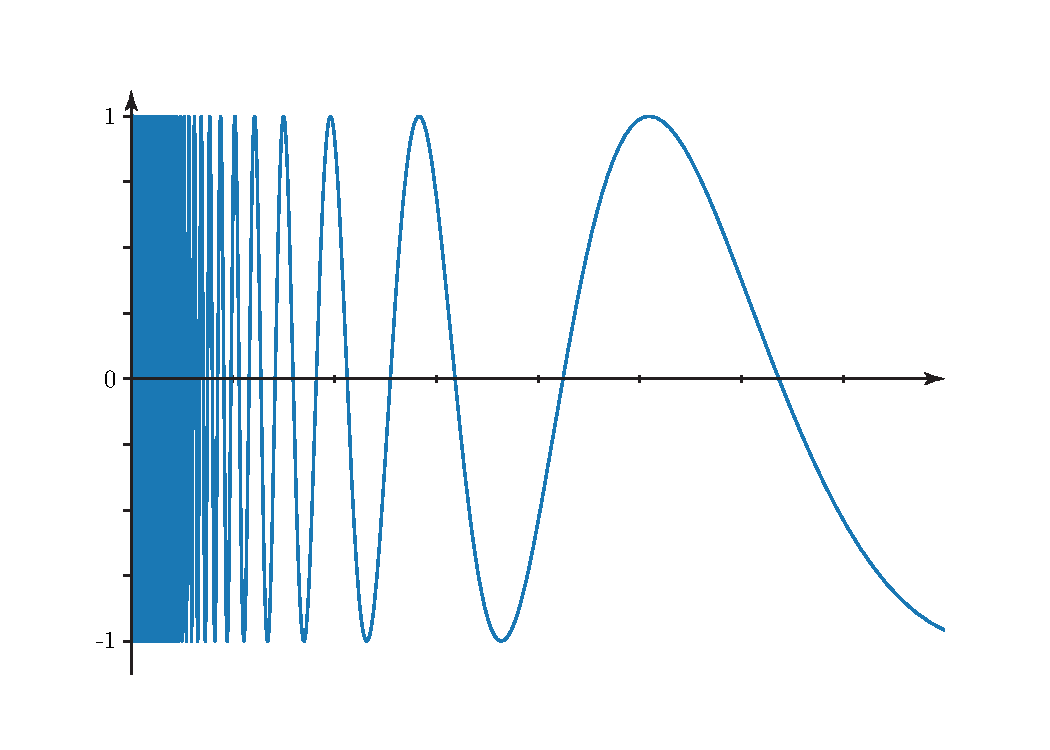
\includegraphics[trim=0cm 0.5cm 0.5cm 1.25cm,clip,scale=0.50]{images/topologistsine.pdf}
\end{minipage}
\end{example}
\vspace{6mm}
\begin{example}{}[La pulce ed il pettine]
	Si consideri il ‘‘pettine'' come il seguente sottospazio di $\R ^2$ con la topologia euclidea:
		\begin{equation*}
			Y= \left\{ (x,\ 0) \mid 0\leq x\leq 1 \right\} \cup \bigcup_{\stackrel{r\in\Q}{ 0\leq r\leq 1}} \left\{ (r,\ y) \mid 0\leq y \leq 1 \right\}
		\end{equation*}
\begin{minipage}{0.62\textwidth}
Presi due punti su $Y$ si possono collegare fra loro scendendo alla base del pettine $\unint$ e risalendo sui ‘‘denti'' di ascissa razionale. Quindi $Y$ è c.p.a., allora $Y$ è connesso e $\overline{Y}=\unint\times \unint$. Si consideri ora la ‘‘pulce'', ossia un punto $P$ di ascissa irrazionale ed ordinata 1, ad esempio $P=\left(\frac{\sqrt{2}}{2},\ 1\right)$. Sia $Z=Y\cup P$; per il teorema precedente segue che $Z$ è connesso, infatti
\begin{equation*}
	Y\subseteq Z \subseteq \overline{Y}=\unint\times \unint	.
\end{equation*}
	\end{minipage}
	\begin{minipage}{0.37\textwidth}
		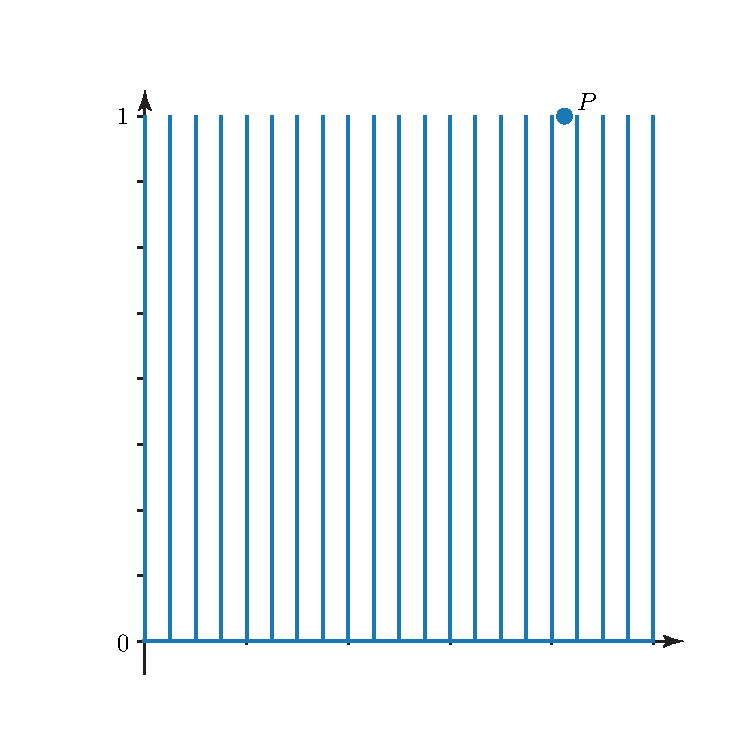
\includegraphics[trim=1.1cm 0.5cm 0.5cm 1.25cm,clip,scale=0.50]{images/comb.pdf}
	\end{minipage}\\
Tuttavia, $Z$ non è c.p.a.: preso un cammino $\funct{}[\alpha]{\unint}{Z\subseteq \R^2}$ tale che $\alpha(t)= \left( x(t), y(t)\right)$ con $\alpha (0)=(0,0)$ e $\alpha(1)=P$, per continuità $y(t)\neq 0 \implies x(t)\in\Q$, ma \textit{non} è vero per $P$ che ha ascissa irrazionale, dunque non esiste un cammino continuo che colleghi l'origine e $P$. Ne consegue che $Z$ \textit{non} è c.p.a..
\end{example}
\subsection{Componenti connesse}
L'intuizione geometrica che ci ha portati alla definizione di connessione è stata ‘‘di quanti pezzi è fatto uno spazio?''. Se uno spazio è connesso è fatto di un solo ‘‘pezzo'', cerchiamo ora di definire cosa sono i ‘‘pezzi'' e come sono fatti.
\begin{definition}{}[Componente connessa]
	Sia $X$ uno spazio topologico e $C\subseteq X$. Si dice che $C$ è una \textbf{componente connessa}\index{componente!connessa} se:
		\begin{itemize}
			\item $C$ è connesso.
			\item $C$ è \textbf{massimale}\index{massimale}, ovvero $C\subseteq A$, $A$ connesso $\implies C=A$.
		\end{itemize}
	Scelto $x\in X$ si può definire la \textbf{componente connessa di un punto}\index{componente!connessa di un punto} come
	\begin{equation}
		\displaystyle C(x)=\bigcup \{C \mid C\text{ connesso},\ x\in C\}.
	\end{equation}
\end{definition}
La componente connessa di \textit{un punto} è effettivamente una componente connessa: infatti, è connessa perché unione di connessi con intersezione \textit{non vuota}, avendo $x$ stesso, e se $C(x)\subseteq A$, allora $x\in A$ e quindi $A\subseteq C(x)$, ossia $A=C(x)$.\\
Vediamo ora qualche proprietà delle componenti connesse, in particolare che sono chiuse e formano una partizione.
\begin{property}{}[Proprietà delle componenti connesse]
	Sia $X$ uno spazio topologico. Allora:
		\begin{enumerate}
			\item le componenti connesse sono chiuse;
			\item le componenti connesse formano una partizione di $X$.
		\end{enumerate}
\end{property}
\begin{proof}{n}~{}
	\begin{enumerate}[label=\Roman*]
		\item Sia $C$ una componente connessa. Per ogni insieme vale che $C\subseteq\overline{C}$, ma $C$ è connesso, quindi $\overline{C}$ è connesso. Siccome $C$ è massimale allora $C=\overline{C}$, ossia è chiuso.
		\item Per dimostrare che le componenti connesse formano una partizione di $X$ dobbiamo mostrare che $X$ è unione disgiunta delle componenti connesse. Prima di tutto, notiamo come l'unione delle componenti connesse $C\left(x\right)$ al variare dei punti $x\in X$ coprono lo spazio:
			\begin{equation*}
				\forall x\in X,\ x\in C(x) \implies X=\bigcup_{x\in X}C(x)
			\end{equation*}
		Mostriamo ora che sono disgiunte. Prendiamo due componenti connesse $C$ e $D$ e supponiamo per assurdo che non siano disgiunte; grazie alla proprietà di massimalità delle componenti connesse segue che:
		\begin{gather*}
			C\cap D\neq\emptyset \implies C\cup D \text{ connesso } \implies C=C\cup D=D\qedhere
		\end{gather*}
	\end{enumerate}
\end{proof}
\begin{example}{}
	Sia $\Q\subseteq\R$ con la topologia Euclidea. La componenti connesse di $\Q$ sono i punti, quindi i punti sono chiusi in $\Q$, il che è una riconferma dato che sappiamo che $\Q$ è Hausdorff. Tuttavia non possono essere aperti altrimenti avremmo la topologia discreta!	Inoltre siccome $\Q$ ha più di una componente connessa significa che non è connesso! Invece $\R$ è connesso grazie all'assioma di completezza.
\end{example}
\begin{remark}{n}
	Dati due spazi omeomorfi si ha che hanno lo stesso numero di componenti connesse in quanto l'immagine continua di connessi è connessa. Quindi il \textbf{numero di componenti connesse} ci fornisce un criterio per determinare quando due spazi non sono omeomorfi!
\end{remark}


		\section{Compattezza}
\begin{definition}{}[Ricoprimento aperto e sottoricoprimento]
	Sia $X$ uno spazio topologico. Un \textbf{ricoprimento aperto}\index{ricoprimento}\index{ricoprimento!aperto} di $X$ è una famiglia $\mathcal{A}=\{A_i \}_{i\in I}$ di aperti di $X$ tali che
	\begin{equation*}
		 X=\bigcup_{i\in I} A_i.
	\end{equation*}
	Un \textbf{sottoricoprimento}\index{sottoricoprimento} $\mathcal{B}$ di un ricoprimento aperto $\mathcal{A}$ è una famiglia di aperti di $\mathcal{A}$ la cui unione è ancora tutto $X$.
\end{definition}		

\begin{example}{pn}[Ricoprimenti aperti]~{}
	\begin{itemize}
		\item $\displaystyle \R=(-\infty ,\ 2)\cup(0,\ +\infty)$ è un ricoprimento aperto
		\item $\displaystyle \R =\bigcup_{n\in\N}(-n,\ n)$ è un ricoprimento aperto
		\item $\displaystyle \R=\bigcup_{p \text{ primo}}(-p,p)$ è un ricoprimento aperto
	\end{itemize}
\end{example}

\begin{definition}{}[Spazio compatto]
	Uno spazio topologico $X$ si dice \textbf{compatto}\index{spazio!compatto} se dato un qualsiasi ricoprimento aperto $\mathcal{A}$ si può sempre estrarre un sottoricoprimento \textit{finito} $\mathcal{B}$.
\end{definition}
L'importanza della definizione risiede nel fatto che non si chiede che esista un ricoprimento $\mathcal{A}$ finito (basterebbe banalmente $X$ stesso che è aperto) bensì che da $\mathcal{A}$ si possa sempre estrarre un \textit{numero finito di aperti} che ricopra ancora $X$.

\begin{example}{pn}[spazi \textit{non} compatti]~{}
	\begin{itemize}
		\item $\R$ con la topologia euclidea: se si considera il ricoprimento aperto $\displaystyle \R=(-\infty , 2)\cup(0,+\infty)$, esso non ammette sottoricoprimento finito.
		\item Gli intervalli aperti o semiaperti della forma $[a,\ b)$ hanno come ricoprimento aperto $\mathcal{A}=\left\{ \left[ a, \ b-\frac{1}{n}\right) \right\}_{n\in \N}$, che non ammette un sottoricoprimento finito.
	\end{itemize}
\end{example}

\begin{theorem}{}[Immagine continua di un compatto è compatta]\label{immagine compatto}
	Dati $X,Y$ spazi topologici, $\funct{}[f]{X}{Y}$ continua, allora
		\begin{gather*}
			X \text{ compatto } \implies f(X) \text{ compatto }
		\end{gather*}
\end{theorem}
\begin{proof}{n}
	Sia  $\mathcal{A}=\{A_i\}$ ricoprimento aperto di $f(X)$. Per definizione di ricoprimento allora:
	\begin{equation*}
		f(X)\subseteq \bigcup_{i\in I}A_i
	\end{equation*}
	Si considerino ora le controimmagini degli aperti $A_i$ tramite $f$, aperte in quanto $f$ è continua.
	\begin{equation*}
	X\subseteq f^{-1}\left(\bigcup_{i\in I}A_i\right)=\bigcup_{i\in I}f^{-1}\left(A_i\right)
	\end{equation*}	
	Da ciò si evince che $\mathcal{A}'=\left\{f^{-1}(A_i)\right\}$ è un ricoprimento aperto di $X$; essendo $X$ compatto, si può estrarre un sottoricoprimento finito di $X$. Riapplicando la funzione $f$ troviamo un sottoricoprimento finito del ricoprimento originale:
	\begin{gather*}
		X=f^{-1}(A_1) \cup	\ldots \cup f^{-1}(A_n) \implies f(X)\subseteq A_1\cup \ldots \cup A_n \implies f(X) \text{ compatto}\qedhere
	\end{gather*}
\end{proof}
Da questo teorema segue che essere compatti è una \textbf{proprietà topologica}.
% LEZ 09
\begin{theorem}{}[{$\unint$} è compatto]
	L'intervallo $\unint\subseteq\R$ con la topologia euclidea è compatto.
\end{theorem}
\begin{proof}{n}
	Sia $\mathcal{A}=\{ A_i\}_{i\in I}$ un ricoprimento aperto di $\unint$ con $A_i$ aperti in $\R$.
	Sia $X\coloneqq \{ t\in\R \mid [0,t] \text{ è coperto da un numero finito di } A_i \}$. Questo insieme \textit{non} è vuoto; infatti, per $t=0$:
		\begin{gather*}
			[0,\ t]=[0,\ 0]=\{0\}\implies\exists A_0\in\mathcal{A}\colon \{0\}\subseteq A_{0} \implies 0\in X\implies X\neq\emptyset
		\end{gather*}
	Siccome $X$ non è vuoto, per la completezza dei reali ne posso considerare l'estremo superiore $b=\sup X$. Ci sono due casi, $b>1$  e $b\leq 1$: dimostriamo che il primo è possibile mentre il secondo è assurdo per definizione di estremo superiore:
		\begin{itemize}
			\item $b>1$: esiste un $t\in X$ tale che $1<t<b$, ma allora$\unint\subseteq [0,\ t] \subseteq A_1\cup \ldots \cup A_n$
			\item $b\leq 1$: $b\in \unint$, dunque esiste $A_0\in\mathcal{A}$ tale che $b\in A_0$ con $A_0$ aperto; per definizione della topologia Euclidea esisterà una palla aperta centrata in $b$ contenuta in $A_0$:
			\begin{equation*}
				\exists \delta >0 \colon B_\delta (b)=(b-\delta, \ b+\delta )\subseteq A_0.
			\end{equation*}
			Sia $0<h<\delta$. Consideriamo $b+h$ e l'intervallo $[0,\ b+h]$:
				\begin{gather*}
					[0,\ b+h]=[0,\ t]\cup [t,\ b+h]\subseteq \underbrace{A_1\cup\ldots\cup A_n}_{t\in X}\cup \underbrace{A_0}_{B_\delta (b)\subseteq A_0}.
				\end{gather*}	
			Quindi $b+h$ è coperto da un numero finito di aperti, pertanto $b+h\in X$, il che è assurdo perché $b=\sup X$.
		\end{itemize}
	 Segue che solo il caso $b>1$ è lecito, da cui si ha che $\unint$ è coperto da un numero finito di aperti del ricoprimento iniziale e quindi è compatto.\qedhere
\end{proof}
Notiamo che questo teorema implica che un intervallo $[a,\ b]\subseteq\R$ è compatto, essendo omeomorfo a $\unint$. Vediamo ora un esempio di spazio compatto che non abbia la topologia euclidea.
\begin{example}{}[Uno spazio $X$ con la topologia cofinita {$CF$} è compatto]
	Ricordiamo che gli aperti nella topologia $CF$ sono i sottoinsiemi il cui complementare è finito, quindi gli aperti sono pari a $X$ privato di un numero finito di punti. Preso un ricoprimento aperto $\mathcal{A}=\{A_i\}$, scegliamo un aperto $A_0=X\setminus\{x_1,\ \ldots,\ x_n\}$. Per ricavare un sottoricoprimento finito di $\mathcal{A}$ è sufficiente considerare, per ogni punto $x_i$ che \textit{non} appartiene all'aperto $A_0$, un aperto del ricoprimento che lo contenga. In questo modo $X=A_0\cup A_1\cup A_n$ e quindi $X$ è compatto.
\end{example}
\begin{remark}{n}
Notiamo che se $X$ è \textbf{finito} allora $X$ è compatto per \textit{qualsiasi} topologia: poiché la sua cardinalità è finita, la sarà anche quella del suo \textit{insieme delle parti}, da cui scelgo gli aperti della topologia; un qualunque ricoprimento sarà necessariamente finito. I casi interessanti di spazi compatti sono quelli il cui insieme di sostegno \textit{non è finito}.\\
Inoltre, se $X$ ha la topologia \textbf{discreta} vale anche il \textit{viceversa}:
	\begin{gather*}
		X \text{ top. discreta } \implies \left( X \text{ compatto } \iff X \text{ finito}\right)
	\end{gather*}
$\rightimplies$ Consideriamo il ricoprimento aperto $\mathcal{A}=\left\{ A_x\right\}_{x\in X}$, con $A_x\coloneqq \{x\}$ aperti in quanto $X$ ha la topologia discreta. Siccome $X$ è compatto allora esiste un sottoricoprimento finito, ovvero un numero finito di aperti di $\mathcal{A}$ che ricopre $X$, ossia
\begin{equation*}
	X=\{x_1\}\cup\{x_2\}\cup\ldots\{x_n\}\implies X=\Set{x_1,\ x_2,\ \ldots,\ x_n}\implies X \text{ finito.}
\end{equation*}

\end{remark}
\subsection{Relazioni fra compattezza e altre proprietà topologiche}
\begin{theorem}{}[Chiuso in un compatto è compatto; Manetti, 4.41.1]\label{chiuso in compatto}
Un chiuso in un compatto è un compatto, ovvero se $X$ è uno spazio topologico compatto, $C\subseteq X$ chiuso allora $C$ è compatto.
\end{theorem}
\begin{proof}{n}
	Sia $\mathcal{A}=\{A_i \}_{i\in I}$ un ricoprimento di $C$. Poiché $C\subseteq X$ è chiuso, $A\coloneqq X\setminus C$ è aperto in $X$: si ha che $\mathcal{A}'=\{A_i,\ A\}$ è un ricoprimento aperto di $X$, ma siccome $X$ è compatto esiste un suo sottoricoprimento finito tale che
		\begin{equation*}
			X=A_1\cup\ldots\cup A_n\cup Al\ \A_i\in\mathcal{A}.
		\end{equation*}
	Segue che
	\begin{equation*}
		C=X\setminus A=A_1\cup\ldots\cup A_n,
	\end{equation*}
	ossia $C$ è compatto.\qedhere
\end{proof}

\begin{lemma}{n}[Unione finita di compatti è un compatto; Manetti, 4.41.2]
\end{lemma}
\begin{proof}{n}
Preso un ricoprimento aperto $\mathcal{A}$ di $K_1\cup\ldots\cup K_n$, estraiamo un sottoricoprimento finito $\widetilde{\mathcal{A}}_i$ per ogni $K_i$ compatto: l'unione $\widetilde{\mathcal{A}}_1\cup\ldots\cup \widetilde{\mathcal{A}}_n$ è un sottoricoprimento finito di $\mathcal{A}$ che copre $K_1\cup\ldots\cup K_n$.\qedhere
\end{proof}
% Vediamo ora una relazione importante fra due proprietà topologiche: compattezza e Hausdorff}.
\begin{theorem}{}[Compatto in un Hausdorff è chiuso; Manetti, 4.48]\label{compatto in hausdorff chiuso}
Se $X$ è di Hausdorff e $K\subseteq X$ è compatto, allora $K$ è chiuso.
\end{theorem}
\begin{proof}{n}
	Per dimostrare che $K$ è chiuso mostriamo che il suo complementare è aperto, in particolare mostrando che sia intorno di ogni suo punto.
	Allora, fissato un $x_0$ arbitrario nel complementare, dovrà esistere un aperto contenente $x_0$, che può coincidere o meno con $X\setminus K$, disgiunto da $K$.
		\begin{equation*}
				K \text{ chiuso } \iff X\setminus K \text{ aperto } \iff \exists A\subseteq X\setminus K \text{ con } A \text{ aperto } \colon x_0\in A \iff A\cap K=\emptyset
		\end{equation*}
	Per ipotesi $X$ è di Hausdorff; fissato $x_0\neq y$ in $X\setminus K$, per ogni $y\in K$ chiaramente $x\neq y$, dunque esisteranno due intorni aperti $U_y\in I(x_0)$ e $V_y\in I(y)$ dipendenti dalla scelta di $y$ tali che $U_y\cap V_y=\emptyset$. Consideriamo allora, al variare di $y$, l'unione di tutti gli intorni aperti $V_y$:
	\begin{equation*}
			V\coloneqq \bigcup_{y\in K}V_y \implies K\subseteq V
	\end{equation*}
	Gli aperti $\{V_y\}$ formano un ricoprimento di $K$, dunque, essendo $K$ compatto, estraiamo un sottoricoprimento $V_{y_1}\cup\ldots\cup V_{y_n}$. Prendiamo allora gli intorni aperti di $x_0$ definiti in precedenza e selezioniamo quelli dati da $y_1,\ \ldots,\ y_n$. Sia
	\begin{equation*}
		U=U_{y_1}\cap\ldots\cap U_{y_n} \in I(x_0)
	\end{equation*}
	Gli aperti $V$ e $U$ per costruzione \textit{non} si intersecano, poiché $V\cap U=\emptyset$, e in particolare $U\cap K=\emptyset$ perché $K\subseteq V$. Allora, per le osservazioni iniziali $U\subseteq X\setminus K$, cioè $X\setminus K$ è intorno di $x_0$. Per l'arbitrarietà di $x_0$, segue che $X\setminus K$ è aperto e quindi $K$ chiuso.\qedhere
\end{proof}
\begin{theorem}{}[Teorema di Heine-Borel in {$\R$}; Manetti, 4.42]\label{compatto chiuso e limitato R}
Un sottospazio $K\subseteq \R$ è compatto se e solo se $K$ è chiuso e limitato.
\end{theorem}
\begin{proof}{n}~{}\\
	$\rightimplies$ Siccome $\R$ è di Hausdorff e $K$ è compatto, per il teorema precedente $K$ è chiuso. Per vedere che è limitato consideriamo un ricoprimento aperto $\mathcal{A}=\left\{ (-n,\ n)\cap K\right\}_{n\in\N}$ di $K$. Siccome è compatto allora esiste un sottoricoprimento finito
	\begin{gather*}
		K\subseteq (-n_1,\ n_1)\cup\ldots\cup(-n_m,\ n_m)
	\end{gather*}
	dunque $K\subseteq (-M,\ M), \ M\coloneqq \max n_i$, quindi $K$ è limitato. \\
	$\leftimplies $ $K$ è limitato, quindi $K\subseteq [-n, \ n]$ che è compatto; poiché $K$ è chiuso per ipotesi e contenuto in un compatto, per il teorema \ref{chiuso in compatto} è anch'esso compatto.\qedhere
\end{proof}
\begin{warning}{n}
	Il teorema precedente \textit{non} afferma che gli unici compatti di $\R$ sono gli intervalli chiusi e limitati! Anche una loro \textit{unione finita} (anche disgiunta) potrebbe esserlo.
\end{warning}
\begin{theorem}{}[Funzione su compatto in $\R$ ha massimo/minimo; Manetti, 4.43]\label{weierstrass}
Sia $\funct{}[f]{X}{\R}$ con $X$ compatto e $\R$ con la topologia euclidea. Se $f$ è continua allora ammette massimo e minimo.
\end{theorem}
\begin{proof}{n}
	Data $f$ continua e $X$ compatto, si ha $f(X)$ compatto; per il teorema precedente ciò equivale al fatto che $f(X)$ è chiuso e limitato. 
	\begin{equation*}
		\left.
		\begin{array}{lcl}
			f\left(x\right)\text{ limitata}&\implies& \sup \left\{f\left(x\right)\right\}<+\infty\\
			f\left(x\right)\text{ chiusa}&\implies& \sup \left\{f\left(x\right)\right\}=\max \left\{f\left(x\right)\right\}\\
		\end{array}
		\right\}
		\implies f\left(x\right)\text{ ammette massimo.}
	\end{equation*}
	Analoga è la dimostrazione per il minimo.\qedhere
\end{proof}

\begin{warning}{n}
	Per poter parlare di massimo e minimo di una funzione c'è bisogno di un \textit{ordinamento} sul codominio; il dominio $X$ potrebbe anche non averne uno!
\end{warning}
Vogliamo ora vedere come si comporta la compattezza rispetto al prodotto, prima però va dimostrato un lemma che ci tornerà utile nella dimostrazione del teorema.
\begin{lemma}{}[Tube lemma]\label{tube lemma}
Siano $X,Y$ spazi topologici con $Y$ compatto, $x_0\in X$ e $A\subseteq X\times Y$ aperto tale che $\{x_0\}\times Y\subseteq A$. Allora esiste un aperto aperto $ U\subseteq X$ con $x_0\in U$ tale che $\{x_0\}\times Y \subseteq U\times Y \subseteq A$
\end{lemma}
\begin{proof}{n}
	L'aperto $A$ si può esprimere come unione di aperti della base della topologia prodotto:
	\begin{equation*}
		A=\bigcup_{i\in I}\left( U_i\times V_i \right)
	\end{equation*}
	con $U_i\subseteq X$, $V_i\subseteq Y$. $\mathcal{U}=\{U_i\times V_i\}_{i\in I}$ è un ricoprimento di $\{x_0\}\times Y$; poiché $\{x_0\}\times Y$ è compatto in quanto omeomorfo a $Y$, esiste un suo sottoricoprimento finito estratto da da $\mathcal{U}$:
	\begin{equation*}
		\{x_0\}\times Y\subseteq (U_1\times V_1)\cup\ldots\cup (U_n\times V_n)
	\end{equation*}
	Poniamo $U\coloneqq U_1\cap\ldots\cap U_n$:
	\begin{equation*}
		\{x_0\}\times Y\subseteq U\times Y \subseteq (U_1\times V_1)	\cup\ldots\cup (U_n\times V_n) \subseteq A
	\end{equation*}
	$U$ è l'aperto che soddisfa la tesi.\qedhere
\end{proof}
\begin{theorem}{}[Prodotto di compatti se e solo se fattori compatti; Manetti, 4.49.2]\label{prodotto compatti}
Due spazi $X,Y$ sono compatti se e solo se $X\times Y$ è compatto.
\end{theorem}
\begin{proof}{n}~{}\\
	$\leftimplies $ Le proiezioni $p$ e $q$ sono funzioni continue e suriettive. Poiché $X\times Y$ è compatto e $p\left(X\times Y\right)=X$ e $q\left(X\times Y\right)=Y$, allora $X,\ Y$ sono compatti. \\
	$\rightimplies $ Sia $\mathcal{A}=\{A_i\}$ un ricoprimento aperto di $X\times Y$. Per ipotesi $Y$ è compatto, dunque per ogni $x\in X$ si ha $\{x\}\times Y$ compatto in quanto $\{x\}\times Y\cong Y$.
	Estraiamo un sottoricoprimento finito da $\mathcal{A}$ che copra $\{x\}\times Y$:
	\begin{equation*}
		\{x\}\times Y\subseteq A_{x,1}\cup\ldots\cup A_{x,n}=A_x
	\end{equation*}
	Gli $A_{x_i}$ dipendono dal punto $x$ scelto. Poiché $A_x$ è aperto, per il \textit{Tube lemma} allora esiste $U_x\subseteq X$ aperto tale che
		\begin{equation*}
			\{ x\}\times Y \subseteq U_x\times Y \subseteq A_x=A_{x,1}\cup\ldots\cup A_{x,n}
		\end{equation*}
	Al variare di $x\in X$ si ha un ricoprimento $\mathcal{U}=\left\{U_x\right\}_{x\in X}$ di $X$ compatto, dunque possiamo estrarne un sottoricoprimento finito $X=U_{x_1}\cup\ldots\cup U_{x_m}$. Usando la proiezione sulla componente $X$:
		\begin{align*}
				X\times Y &= p^{-1}(X)=p^{-1}\left( U_{x_1}\cup\ldots\cup U_{x_m}\right)= (U_{x_1}\times Y)\cup\ldots\cup (U_{x_m}\times Y)\\
				&\subseteq A_{x_1}\cup\ldots\cup A_{x_m} 
				\subseteq \left( A_{x_1 , 1}\cup\ldots\cup A_{x_1, n_1}\right) \cup\ldots\cup \left( A_{x_m, 1}\cup\ldots\cup A_{x_m, n_m} \right)
		\end{align*}
	Poichè $X\times Y$ è coperto da un unione finita di un unione finita di aperti del ricoprimento $\mathcal{A}$, segue che è compatto.\qedhere
\end{proof}
Noto che il prodotto di compatti è compatto, possiamo generalizzare la caratterizzazione dei compatti in $\R$ (teorema \ref{compatto chiuso e limitato R}) al caso dello spazio $\R^n$.
\begin{theorem}{}[Teorema di Heine-Borel in {$\R^n$}; Manetti, 4.42]\label{compatto chiuso e limitato R^n}
Un insieme $K\subseteq \R^n$ è compatto se e solo se $K$ è chiuso e limitato.
\end{theorem}
\begin{proof}{n}~{}\\
	$\rightimplies$ $K$ è compatto in $\R^n$ che è Hausdorff, quindi $K$ è chiuso per il teorema \ref{compatto in hausdorff chiuso} (Manetti, 4.48). Per dimostrare che è limitato consideriamo un ricoprimento di palle aperte centrate nell'origine e utilizziamo l'ipotesi di $K$ compatto:
		\begin{gather*}
			K\subseteq \bigcup_{n\in\N} B_n(\mathbf{0}) \implies K\subseteq B_{n_1}(\mathbf{0})\cup\ldots\cup B_{n_m}(\mathbf{0}) \subseteq B_M (\mathbf{0})
		\end{gather*}
	con $M=\max n_i$.\\
	$\leftimplies$ $K$ è limitato, quindi $K\subseteq [-a,\ a]^n$ che è compatto perché prodotto di compatti. Essendo $K$ chiuso, per il teorema \ref{chiuso in compatto} (Manetti, 4.41.1) è compatto.\qedhere
\end{proof}
\begin{digression}{}
In realtà vale un teorema più generale, che si dimostrerà poi nel corso di \textit{Istituzioni di Analisi}: dato uno spazio metrico \textit{completo} $X$, allora $K\subseteq X$ compatto se e solo se $K$ chiuso e \textbf{totalmente limitato}\index{spazio!totalmente limitato}, cioè $\forall\epsilon >0, \ K$ è contenuto in un'unione finita di palle di raggio $\epsilon$. In $\R^n$ limitato e totalmente limitato sono equivalenti, ma in generale no; ad esempio, consideriamo lo spazio metrico delle funzioni continue su $\unint$ con distanza dell'estremo superiore:
	\begin{equation*}
		\mathcal{C}\left( \unint \right) \coloneqq \left\{ \funct{}[f]{\unint}{\R} \mid f \text{ continua } \right\},  \ \ \text{con } d\left(f,g\right) =\sup_{x\in \unint} |f(x)-g(x)|
	\end{equation*}
La palla di centro l'origine $0$ e raggio $1$
\begin{equation*}
	B_1(\mathbf{0})=\left\{ \funct{}[f]{\unint}{\R} \mid f \text{ continua }, -1\geq f(x) \leq 1 \ \right\}
\end{equation*}
è chiusa e limitata, tuttavia in $\mathcal{C}\left( \unint \right)$ non è compatta.
\end{digression}
\begin{theorem}{}[Funzione continua da compatto ad Hausdorff è chiusa; Manetti, 4.52]\label{da compatto in T_2 è chiuso}
Se $\funct{}[f]{X}{Y}$ continua con $X$ è compatto e $Y$ di Hausdorff, allora $f$ è chiusa.
\end{theorem}
\begin{proof}{n}
	Per mostrare che $f$ è chiusa consideriamo $C\subseteq X$ chiuso e mostriamo che $f(C)$ è chiuso usando i teoremi \ref{chiuso in compatto}, \ref{immagine compatto} e \ref{compatto in hausdorff chiuso}. $C\subseteq X$ è un chiuso in un compatto, dunque $C$ è compatto e pertanto lo è la sua immagine $f(C)$ che è contenuta in $Y$ di Hausdorff, dunque $f(C)$ è chiuso.
\end{proof}
In generale vale il
\begin{theorem}{q}[Kuratowski-Mròwka]
	$Y$ è compatto se e solo se per qualsiasi spazio topologico $X$ la proiezione $\funct{}[p_X]{X\times Y}{X}$ è chiusa.\qedhere
\end{theorem}
Noi ne dimostriamo una versione più debole.
% LEZ 10
\begin{theorem}{}[Prodotto con compatto implica proiezione chiusa; Manetti, 4.49.1]
Siano $X,\ Y$ spazi topologici con $Y$ compatto, allora la proiezione $\funct{}[p]{X\times Y}{X}$ è chiusa.
\end{theorem}
\begin{proof}{n}
	Preso $C\subseteq X\times Y$ chiuso, vogliamo mostrare che $p(C)\subseteq X$ è chiuso. Per far ciò, mostriamo che il suo complementare $X\setminus p(C)$ è aperto in quanto intorno di ogni suo punto. Chiaramente, se $p(C)=X$ allora è già chiuso; se invece $p(C)\neq X$, allora esiste $x_0\in X\setminus p(C)$. Si consideri la fibra di $x_0$ tramite la proiezione $p$:
		\begin{gather*}
			p^{-1}(\{x_0\} )=\{x_0\}\times Y \subseteq (X\times Y)\setminus C,
		\end{gather*}
	con $(X\times Y)\setminus C$ aperto perché complementare in $X\times Y$ del chiuso $C$. Valgono le ipotesi del \textit{Tube Lemma}: esiste $U\subseteq X$ aperto tale che
		\begin{equation*}
			\colon \{x_0\}\times Y \subseteq U\times Y\subseteq (X\times Y)\setminus C.
		\end{equation*}
	Poiché la proiezione è continua, si ha
	\begin{equation*}
			p^{-1}(U)=U\times Y\subseteq (X\times Y)\setminus C \implies p^{-1}(U)\cap C=\emptyset\implies U\cap p(C)=\emptyset
	\end{equation*}
Allora $x_0\in U\subseteq X\setminus p(C)$, dunque $X\setminus p\left(C\right)$ è intorno di $x_0$. Poiché questo è vero per ogni $ x_0\in X\setminus p\left(C\right)$, $X\setminus p\left(C\right)$ è intorno di ogni suo punto, quindi aperto. Segue pertanto la tesi.\qedhere
\end{proof}